\setcounter{page}{14}
\twocolumn

\vspace*{2.5cm}

\noindent \textit{И. Быстрый} \\

\noindent \textbf{\huge Площадь сегмента параболы Нейля}

\vspace{1cm}
\noindent В 1657 году двадцатилетний студент Оксфордского университета Уильям Нейль (1637--1670) нашел длину дуги <<полукубической параболы>> $y=a \sqrt[3]{x^2}$. Это открытие поразило современников, и в память о рано умершем талантливом математике полукубическая парабола называется \textit{параболой Нейля}.

В наше время параболу Нейля можно встретить не только в вузовском курсе анализа, но и в школьном учебнике\footnote{<<Алгебра и начала анализа 9>>, задачи 438, 474б, <<Алгебра и начала анализа 10>>, задача 393а}). А недавно на лекции для абитуриентов я получил такую записку:

\textit{Как найти площадь фигуры, ограниченной кривой $y=3 \sqrt[3]{x^2}$ и касательной к ней в точке $x=-8$?}

Вот что я тогда ответил.

Эта задача, несмотря на кажущуюся простоту, связана с определенными трудностями. Первая трудность возникает при нахождении касательной к параболе Нейля
\vspace{-5pt}
\begin{align}
    f_1(x) &= 3 \sqrt[3]{x^2} \label{eq:f1}
\end{align}
в точке $x=-8$. Как известно, уравнение касательной определяется по формуле
\vspace{-5pt}
\begin{align}
y-f_1(-8)=f_1'(-8)(x+8). \label{eq:f2}
\end{align}
Здесь
\vspace{-10pt}
\begin{align*}
    f_1(-8)=12,
\end{align*}
\begin{align*}
    f_1'(-8) &= 3(x^{\frac{2}{3}})'|_{x=-8} = \\
    &= 3 \cdot \frac{2}{3}x^{- \frac{2}{3}}|_{x=-8}=2\cdot (-8) ^ {- \frac{1}{3}}.
\end{align*}
Значит, производная не существует (поскольку выражение $(-8)^{- \frac{1}{3}}$ не имеет смысла), следовательно, не существует и касательной к кривой (1).

Между тем, из чертежа ясно, что вывод неверен: прямая $(AB)$ -- касательная! В чем дело? Как же найти угловой коэффициент касательной? Дело в том, что формула 
\vspace{-5pt}
\begin{align*}
    (\sqrt[n]{x^m})'=(x^{\frac{m}{n}})'=\frac{m}{n}x^{\frac{m}{n}-1},
\end{align*}
верная при $x \geq 0$, здесь неприменима. Для вычисления производной (при $x<0$) следует пользоваться формулой
\vspace{-5pt}
\begin{align}
    (\sqrt[n]{x^m})'=\frac{m}{n}\frac{\sqrt[n]{x^m}}{x}, \tag{*} \\
    x \neq 0, n \in \mathbb{N}, m \in \mathbb{Z}. \notag
\end{align}
(которая, разумеется, применима и для положительных $x$). В соответствии с ней имеем
\vspace{-5pt}
\begin{align*}
    f_1'(-8)=(3\sqrt[3]{x^2})&'|_{x=-8}=\\
    &=3\cdot\frac{2}{3}\frac{\sqrt[3]{(-8)^2}}{(-8)}=-1
\end{align*}
Подставив $f_1(-8)=12$ и $f_1(-8)=-1$ в равенство (\ref{eq:f2}), получим искомое уравнение касательной 
\vspace{-5pt}
\begin{align*}
    y=4-x.
\end{align*}

У п р а ж н е н и е 1. \textit{Найдите точки пересечения линий $f_1(x)=3\sqrt[3]{x^2}$ и $f_2(x)=4-x$}.

Теперь, когда известна абсцисса точки $B$, легко найти площадь криволинейного треугольника $AOB$.

\vspace{0.5cm}
\begin{figure}[h]
    \centering
    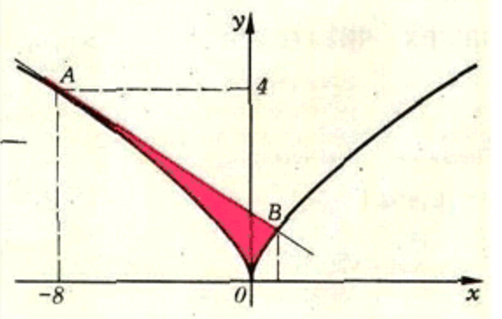
\includegraphics[width=1\linewidth]{latex21111.png}
    \label{fig:enter-label}
\end{figure}